% !TeX root = thesis.tex
\documentclass{master_thesis}
\addbibresource{refs.bib}

\begin{document}

\section{Results}

% This section should have answers to all my research questions
% Follow up survey + reach out to dev's I know have used addon-a11y

\subsection{Comparing results from manual audit and automated report}

To get the whole list including all components a report was created that included the violations caught in each example of each component. This report was generated at the beginning of the manual audit, so the results obtained from both methods are based on the same source code.
\begin{figure}[H]
	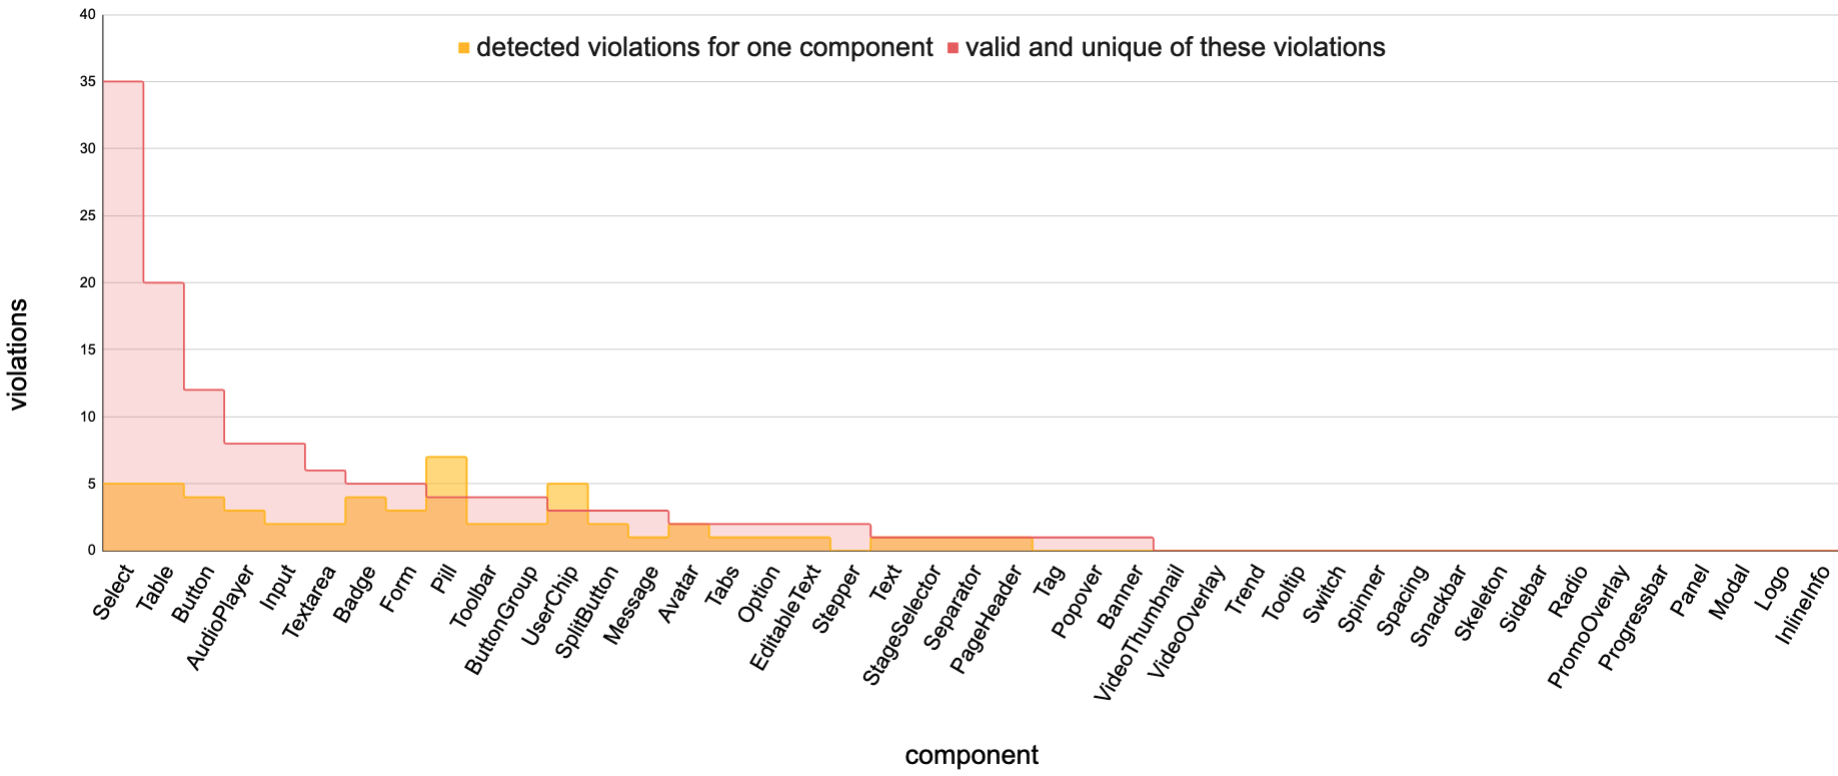
\includegraphics[width=\textwidth]{img/audit-failed.png}
	\caption{All violation found by addon-a11y and how many of them are valid.}
	\label{fig:audit-failed}
\end{figure}

I prepared a comparison table form both results. For automated accessibility tests I recorded the number of examples that included violations, the number of different violations and the number of passed checks for each component. In most cases there were more examples with violations because the same thing was reported in more than one example (see figure \ref{fig:audit-failed}). Addon-a11y did not report any issues for 27 components out of 53 components.

\begin{figure}[H]
	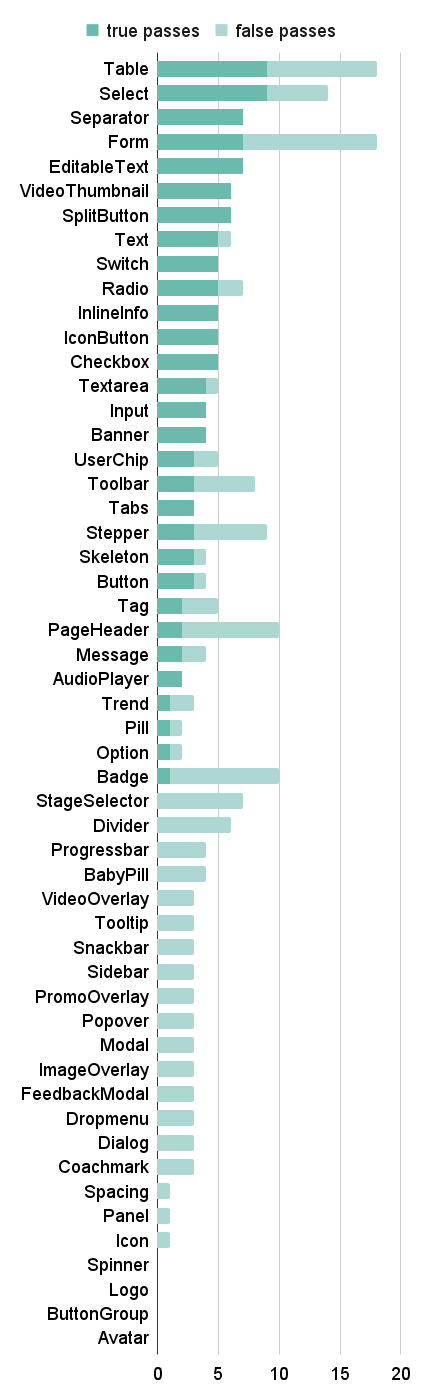
\includegraphics[width=\textwidth]{img/audit-passed.png}
	\caption{All passed checks reported by addon-a11y and how many of them are valid. }
	\label{fig:audit-passed}
\end{figure}
Passed issues where looked over to determine how many where valid (see figure \ref{fig:audit-passed}). 4 components did not have any passed issues and 22 did not have any valid passed issues.

Looking at all the fails and passes gives an overview of what was checked for each component. Out of 53 components only 2 did not get checked by addon-a11y at all. In addition, components that become visible only when triggered by another element, like modals and popups that currently in our library displayed with a button as a trigger, don't get tested. These components are seen on figure \ref{fig:audit-passed} starting from \textit{VideoOverlay} and ending with \textit{Coachmark} - 27 over all. This means 29 components where not tested but this tool and rest of the components had passed or failed issues, but often not both.

\begin{figure}[H]
	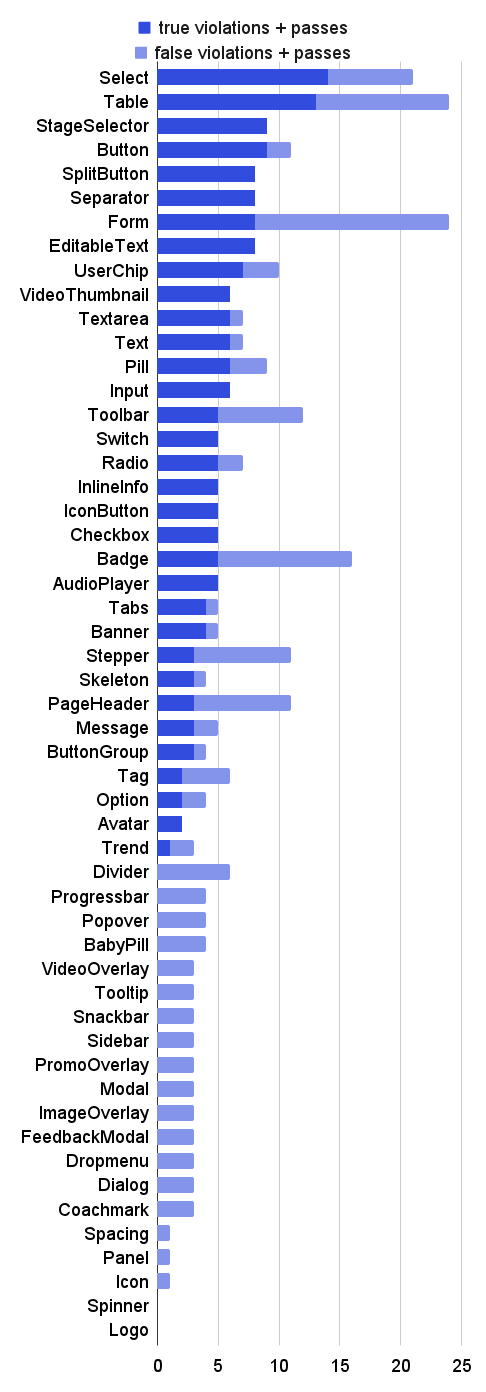
\includegraphics[width=\textwidth]{img/audit-all.png}
	\caption{All issues that where tested by addon-a11y. This means both passed and failed issues combined.}
	\label{fig:audit-all}
\end{figure}

In some cases there were 0 violations detected, and 0 valid checks passed – this means that the automated testing was not effective (\todo{Make chart or table for this}).

\subsection{Limitations of using Storybook's addon-a11y}

The accessibility add-on in Storybook analyzes the examples that have been made for the component and unsuitable example can cause false results. Like Components triggered by a button described before. This is because the initial HTML that the accessibility tests are being run on only has the button and the tests are not being run again after triggering the element. This could potentially be remedied with better examples.

The biggest limitation of this tool currently is that it can only be view-d in storybook. To see the number of passes and fails you need to open the accessibility tab for each component. I looked into ways of automating this so that the same checks could be run on every change to the library and added to continuous integration (CI) workflow. In the current version of Storybook there is no easy way to do this, but it will become much easier in the next major version.

Upgrading out component library to that version need some extra work to make it compatible, but I have tested out this solution on a test library, and it seems like it would definitely be an improvement. Running the tests in CI would ensure that they are run every time someone makes a change and not only when we choose to. We could also block changes that don't pass the required accessibility checks.

\todo{Reasons for automated check not being effective}



\end{document}